% Created by tikzDevice version 0.12.6 on 2024-03-15 15:16:53
% !TEX encoding = UTF-8 Unicode
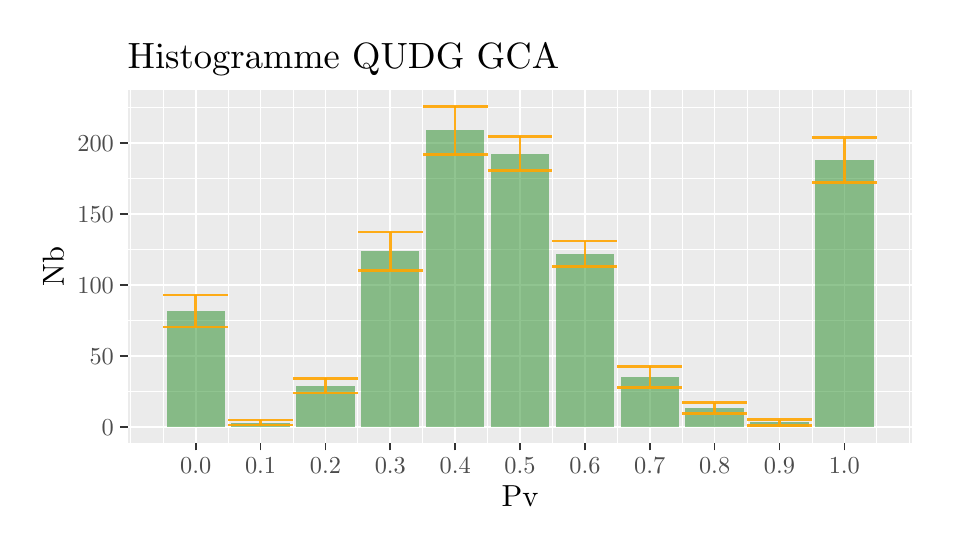
\begin{tikzpicture}[x=1pt,y=1pt]
\definecolor{fillColor}{RGB}{255,255,255}
\path[use as bounding box,fill=fillColor,fill opacity=0.00] (0,0) rectangle (325.21,180.67);
\begin{scope}
\path[clip] (  0.00,  0.00) rectangle (325.21,180.67);
\definecolor{drawColor}{RGB}{255,255,255}
\definecolor{fillColor}{RGB}{255,255,255}

\path[draw=drawColor,line width= 0.6pt,line join=round,line cap=round,fill=fillColor] (  0.00,  0.00) rectangle (325.21,180.68);
\end{scope}
\begin{scope}
\path[clip] ( 36.11, 30.69) rectangle (319.71,158.02);
\definecolor{fillColor}{gray}{0.92}

\path[fill=fillColor] ( 36.11, 30.69) rectangle (319.71,158.02);
\definecolor{drawColor}{RGB}{255,255,255}

\path[draw=drawColor,line width= 0.3pt,line join=round] ( 36.11, 49.29) --
	(319.71, 49.29);

\path[draw=drawColor,line width= 0.3pt,line join=round] ( 36.11, 74.91) --
	(319.71, 74.91);

\path[draw=drawColor,line width= 0.3pt,line join=round] ( 36.11,100.54) --
	(319.71,100.54);

\path[draw=drawColor,line width= 0.3pt,line join=round] ( 36.11,126.16) --
	(319.71,126.16);

\path[draw=drawColor,line width= 0.3pt,line join=round] ( 36.11,151.79) --
	(319.71,151.79);

\path[draw=drawColor,line width= 0.3pt,line join=round] ( 37.28, 30.69) --
	( 37.28,158.02);

\path[draw=drawColor,line width= 0.3pt,line join=round] ( 49.00, 30.69) --
	( 49.00,158.02);

\path[draw=drawColor,line width= 0.3pt,line join=round] ( 72.44, 30.69) --
	( 72.44,158.02);

\path[draw=drawColor,line width= 0.3pt,line join=round] ( 95.88, 30.69) --
	( 95.88,158.02);

\path[draw=drawColor,line width= 0.3pt,line join=round] (119.32, 30.69) --
	(119.32,158.02);

\path[draw=drawColor,line width= 0.3pt,line join=round] (142.76, 30.69) --
	(142.76,158.02);

\path[draw=drawColor,line width= 0.3pt,line join=round] (166.19, 30.69) --
	(166.19,158.02);

\path[draw=drawColor,line width= 0.3pt,line join=round] (189.63, 30.69) --
	(189.63,158.02);

\path[draw=drawColor,line width= 0.3pt,line join=round] (213.07, 30.69) --
	(213.07,158.02);

\path[draw=drawColor,line width= 0.3pt,line join=round] (236.51, 30.69) --
	(236.51,158.02);

\path[draw=drawColor,line width= 0.3pt,line join=round] (259.95, 30.69) --
	(259.95,158.02);

\path[draw=drawColor,line width= 0.3pt,line join=round] (283.39, 30.69) --
	(283.39,158.02);

\path[draw=drawColor,line width= 0.3pt,line join=round] (306.82, 30.69) --
	(306.82,158.02);

\path[draw=drawColor,line width= 0.3pt,line join=round] (318.54, 30.69) --
	(318.54,158.02);

\path[draw=drawColor,line width= 0.6pt,line join=round] ( 36.11, 36.47) --
	(319.71, 36.47);

\path[draw=drawColor,line width= 0.6pt,line join=round] ( 36.11, 62.10) --
	(319.71, 62.10);

\path[draw=drawColor,line width= 0.6pt,line join=round] ( 36.11, 87.72) --
	(319.71, 87.72);

\path[draw=drawColor,line width= 0.6pt,line join=round] ( 36.11,113.35) --
	(319.71,113.35);

\path[draw=drawColor,line width= 0.6pt,line join=round] ( 36.11,138.97) --
	(319.71,138.97);

\path[draw=drawColor,line width= 0.6pt,line join=round] ( 60.72, 30.69) --
	( 60.72,158.02);

\path[draw=drawColor,line width= 0.6pt,line join=round] ( 84.16, 30.69) --
	( 84.16,158.02);

\path[draw=drawColor,line width= 0.6pt,line join=round] (107.60, 30.69) --
	(107.60,158.02);

\path[draw=drawColor,line width= 0.6pt,line join=round] (131.04, 30.69) --
	(131.04,158.02);

\path[draw=drawColor,line width= 0.6pt,line join=round] (154.47, 30.69) --
	(154.47,158.02);

\path[draw=drawColor,line width= 0.6pt,line join=round] (177.91, 30.69) --
	(177.91,158.02);

\path[draw=drawColor,line width= 0.6pt,line join=round] (201.35, 30.69) --
	(201.35,158.02);

\path[draw=drawColor,line width= 0.6pt,line join=round] (224.79, 30.69) --
	(224.79,158.02);

\path[draw=drawColor,line width= 0.6pt,line join=round] (248.23, 30.69) --
	(248.23,158.02);

\path[draw=drawColor,line width= 0.6pt,line join=round] (271.67, 30.69) --
	(271.67,158.02);

\path[draw=drawColor,line width= 0.6pt,line join=round] (295.10, 30.69) --
	(295.10,158.02);
\definecolor{fillColor}{RGB}{34,139,34}

\path[fill=fillColor,fill opacity=0.50] ( 50.17, 36.47) rectangle ( 71.27, 78.32);

\path[fill=fillColor,fill opacity=0.50] ( 73.61, 36.47) rectangle ( 94.71, 37.91);

\path[fill=fillColor,fill opacity=0.50] ( 97.05, 36.47) rectangle (118.15, 51.32);

\path[fill=fillColor,fill opacity=0.50] (120.49, 36.47) rectangle (141.58, 99.88);

\path[fill=fillColor,fill opacity=0.50] (143.93, 36.47) rectangle (165.02,143.53);

\path[fill=fillColor,fill opacity=0.50] (167.37, 36.47) rectangle (188.46,135.20);

\path[fill=fillColor,fill opacity=0.50] (190.80, 36.47) rectangle (211.90, 98.95);

\path[fill=fillColor,fill opacity=0.50] (214.24, 36.47) rectangle (235.34, 54.48);

\path[fill=fillColor,fill opacity=0.50] (237.68, 36.47) rectangle (258.78, 43.27);

\path[fill=fillColor,fill opacity=0.50] (261.12, 36.47) rectangle (282.21, 38.02);

\path[fill=fillColor,fill opacity=0.50] (284.56, 36.47) rectangle (305.65,132.83);
\definecolor{drawColor}{RGB}{255,165,0}

\path[draw=drawColor,draw opacity=0.90,line width= 0.9pt,line join=round] ( 49.00, 84.07) --
	( 72.44, 84.07);

\path[draw=drawColor,draw opacity=0.90,line width= 0.9pt,line join=round] ( 60.72, 84.07) --
	( 60.72, 72.56);

\path[draw=drawColor,draw opacity=0.90,line width= 0.9pt,line join=round] ( 49.00, 72.56) --
	( 72.44, 72.56);

\path[draw=drawColor,draw opacity=0.90,line width= 0.9pt,line join=round] ( 72.44, 38.81) --
	( 95.88, 38.81);

\path[draw=drawColor,draw opacity=0.90,line width= 0.9pt,line join=round] ( 84.16, 38.81) --
	( 84.16, 37.02);

\path[draw=drawColor,draw opacity=0.90,line width= 0.9pt,line join=round] ( 72.44, 37.02) --
	( 95.88, 37.02);

\path[draw=drawColor,draw opacity=0.90,line width= 0.9pt,line join=round] ( 95.88, 53.98) --
	(119.32, 53.98);

\path[draw=drawColor,draw opacity=0.90,line width= 0.9pt,line join=round] (107.60, 53.98) --
	(107.60, 48.65);

\path[draw=drawColor,draw opacity=0.90,line width= 0.9pt,line join=round] ( 95.88, 48.65) --
	(119.32, 48.65);

\path[draw=drawColor,draw opacity=0.90,line width= 0.9pt,line join=round] (119.32,106.89) --
	(142.76,106.89);

\path[draw=drawColor,draw opacity=0.90,line width= 0.9pt,line join=round] (131.04,106.89) --
	(131.04, 92.88);

\path[draw=drawColor,draw opacity=0.90,line width= 0.9pt,line join=round] (119.32, 92.88) --
	(142.76, 92.88);

\path[draw=drawColor,draw opacity=0.90,line width= 0.9pt,line join=round] (142.76,152.23) --
	(166.19,152.23);

\path[draw=drawColor,draw opacity=0.90,line width= 0.9pt,line join=round] (154.47,152.23) --
	(154.47,134.83);

\path[draw=drawColor,draw opacity=0.90,line width= 0.9pt,line join=round] (142.76,134.83) --
	(166.19,134.83);

\path[draw=drawColor,draw opacity=0.90,line width= 0.9pt,line join=round] (166.19,141.36) --
	(189.63,141.36);

\path[draw=drawColor,draw opacity=0.90,line width= 0.9pt,line join=round] (177.91,141.36) --
	(177.91,129.04);

\path[draw=drawColor,draw opacity=0.90,line width= 0.9pt,line join=round] (166.19,129.04) --
	(189.63,129.04);

\path[draw=drawColor,draw opacity=0.90,line width= 0.9pt,line join=round] (189.63,103.62) --
	(213.07,103.62);

\path[draw=drawColor,draw opacity=0.90,line width= 0.9pt,line join=round] (201.35,103.62) --
	(201.35, 94.29);

\path[draw=drawColor,draw opacity=0.90,line width= 0.9pt,line join=round] (189.63, 94.29) --
	(213.07, 94.29);

\path[draw=drawColor,draw opacity=0.90,line width= 0.9pt,line join=round] (213.07, 58.30) --
	(236.51, 58.30);

\path[draw=drawColor,draw opacity=0.90,line width= 0.9pt,line join=round] (224.79, 58.30) --
	(224.79, 50.67);

\path[draw=drawColor,draw opacity=0.90,line width= 0.9pt,line join=round] (213.07, 50.67) --
	(236.51, 50.67);

\path[draw=drawColor,draw opacity=0.90,line width= 0.9pt,line join=round] (236.51, 45.21) --
	(259.95, 45.21);

\path[draw=drawColor,draw opacity=0.90,line width= 0.9pt,line join=round] (248.23, 45.21) --
	(248.23, 41.33);

\path[draw=drawColor,draw opacity=0.90,line width= 0.9pt,line join=round] (236.51, 41.33) --
	(259.95, 41.33);

\path[draw=drawColor,draw opacity=0.90,line width= 0.9pt,line join=round] (259.95, 39.08) --
	(283.39, 39.08);

\path[draw=drawColor,draw opacity=0.90,line width= 0.9pt,line join=round] (271.67, 39.08) --
	(271.67, 36.96);

\path[draw=drawColor,draw opacity=0.90,line width= 0.9pt,line join=round] (259.95, 36.96) --
	(283.39, 36.96);

\path[draw=drawColor,draw opacity=0.90,line width= 0.9pt,line join=round] (283.39,140.90) --
	(306.82,140.90);

\path[draw=drawColor,draw opacity=0.90,line width= 0.9pt,line join=round] (295.10,140.90) --
	(295.10,124.76);

\path[draw=drawColor,draw opacity=0.90,line width= 0.9pt,line join=round] (283.39,124.76) --
	(306.82,124.76);
\end{scope}
\begin{scope}
\path[clip] (  0.00,  0.00) rectangle (325.21,180.67);
\definecolor{drawColor}{gray}{0.30}

\node[text=drawColor,anchor=base east,inner sep=0pt, outer sep=0pt, scale=  0.88] at ( 31.16, 33.44) {0};

\node[text=drawColor,anchor=base east,inner sep=0pt, outer sep=0pt, scale=  0.88] at ( 31.16, 59.07) {50};

\node[text=drawColor,anchor=base east,inner sep=0pt, outer sep=0pt, scale=  0.88] at ( 31.16, 84.69) {100};

\node[text=drawColor,anchor=base east,inner sep=0pt, outer sep=0pt, scale=  0.88] at ( 31.16,110.32) {150};

\node[text=drawColor,anchor=base east,inner sep=0pt, outer sep=0pt, scale=  0.88] at ( 31.16,135.94) {200};
\end{scope}
\begin{scope}
\path[clip] (  0.00,  0.00) rectangle (325.21,180.67);
\definecolor{drawColor}{gray}{0.20}

\path[draw=drawColor,line width= 0.6pt,line join=round] ( 33.36, 36.47) --
	( 36.11, 36.47);

\path[draw=drawColor,line width= 0.6pt,line join=round] ( 33.36, 62.10) --
	( 36.11, 62.10);

\path[draw=drawColor,line width= 0.6pt,line join=round] ( 33.36, 87.72) --
	( 36.11, 87.72);

\path[draw=drawColor,line width= 0.6pt,line join=round] ( 33.36,113.35) --
	( 36.11,113.35);

\path[draw=drawColor,line width= 0.6pt,line join=round] ( 33.36,138.97) --
	( 36.11,138.97);
\end{scope}
\begin{scope}
\path[clip] (  0.00,  0.00) rectangle (325.21,180.67);
\definecolor{drawColor}{gray}{0.20}

\path[draw=drawColor,line width= 0.6pt,line join=round] ( 60.72, 27.94) --
	( 60.72, 30.69);

\path[draw=drawColor,line width= 0.6pt,line join=round] ( 84.16, 27.94) --
	( 84.16, 30.69);

\path[draw=drawColor,line width= 0.6pt,line join=round] (107.60, 27.94) --
	(107.60, 30.69);

\path[draw=drawColor,line width= 0.6pt,line join=round] (131.04, 27.94) --
	(131.04, 30.69);

\path[draw=drawColor,line width= 0.6pt,line join=round] (154.47, 27.94) --
	(154.47, 30.69);

\path[draw=drawColor,line width= 0.6pt,line join=round] (177.91, 27.94) --
	(177.91, 30.69);

\path[draw=drawColor,line width= 0.6pt,line join=round] (201.35, 27.94) --
	(201.35, 30.69);

\path[draw=drawColor,line width= 0.6pt,line join=round] (224.79, 27.94) --
	(224.79, 30.69);

\path[draw=drawColor,line width= 0.6pt,line join=round] (248.23, 27.94) --
	(248.23, 30.69);

\path[draw=drawColor,line width= 0.6pt,line join=round] (271.67, 27.94) --
	(271.67, 30.69);

\path[draw=drawColor,line width= 0.6pt,line join=round] (295.10, 27.94) --
	(295.10, 30.69);
\end{scope}
\begin{scope}
\path[clip] (  0.00,  0.00) rectangle (325.21,180.67);
\definecolor{drawColor}{gray}{0.30}

\node[text=drawColor,anchor=base,inner sep=0pt, outer sep=0pt, scale=  0.88] at ( 60.72, 19.68) {0.0};

\node[text=drawColor,anchor=base,inner sep=0pt, outer sep=0pt, scale=  0.88] at ( 84.16, 19.68) {0.1};

\node[text=drawColor,anchor=base,inner sep=0pt, outer sep=0pt, scale=  0.88] at (107.60, 19.68) {0.2};

\node[text=drawColor,anchor=base,inner sep=0pt, outer sep=0pt, scale=  0.88] at (131.04, 19.68) {0.3};

\node[text=drawColor,anchor=base,inner sep=0pt, outer sep=0pt, scale=  0.88] at (154.47, 19.68) {0.4};

\node[text=drawColor,anchor=base,inner sep=0pt, outer sep=0pt, scale=  0.88] at (177.91, 19.68) {0.5};

\node[text=drawColor,anchor=base,inner sep=0pt, outer sep=0pt, scale=  0.88] at (201.35, 19.68) {0.6};

\node[text=drawColor,anchor=base,inner sep=0pt, outer sep=0pt, scale=  0.88] at (224.79, 19.68) {0.7};

\node[text=drawColor,anchor=base,inner sep=0pt, outer sep=0pt, scale=  0.88] at (248.23, 19.68) {0.8};

\node[text=drawColor,anchor=base,inner sep=0pt, outer sep=0pt, scale=  0.88] at (271.67, 19.68) {0.9};

\node[text=drawColor,anchor=base,inner sep=0pt, outer sep=0pt, scale=  0.88] at (295.10, 19.68) {1.0};
\end{scope}
\begin{scope}
\path[clip] (  0.00,  0.00) rectangle (325.21,180.67);
\definecolor{drawColor}{RGB}{0,0,0}

\node[text=drawColor,anchor=base,inner sep=0pt, outer sep=0pt, scale=  1.10] at (177.91,  7.64) {Pv};
\end{scope}
\begin{scope}
\path[clip] (  0.00,  0.00) rectangle (325.21,180.67);
\definecolor{drawColor}{RGB}{0,0,0}

\node[text=drawColor,rotate= 90.00,anchor=base,inner sep=0pt, outer sep=0pt, scale=  1.10] at ( 13.08, 94.35) {Nb};
\end{scope}
\begin{scope}
\path[clip] (  0.00,  0.00) rectangle (325.21,180.67);
\definecolor{drawColor}{RGB}{0,0,0}

\node[text=drawColor,anchor=base west,inner sep=0pt, outer sep=0pt, scale=  1.32] at ( 36.11,166.08) {Histogramme QUDG GCA};
\end{scope}
\end{tikzpicture}
